\subsubsection{Schichtenmodell}
Eine der gängigsten Arten der Kommunikation findet heutzutage über das Internet statt. 
Dabei handelt es sich um ein weltweit verbundenes Netz von Rechnern. Zur Gewährleistung einer effizienten und geregelten Datenübertragung der heterogenen Computer im Internet wurden Regelwerke, die sogenannten Netzwerkprotokolle, benötigt.
Um das Jahr 1980 wurden daraufhin von verschiedenen Computerherstellern modularisierte Protokolle entwickelt, die fortan als Standard für die digitale Übertragung innerhalb von Rechnernetzen gelten sollen \cite{wikiNetzwerkprotokolle}.
Es musste eine Vielzahl von Aufgaben bewältigt und Anforderung bezüglich Zuverlässigkeit, Sicherheit, Effizienz etc. erfüllt werden. Die Aufgaben reichten dabei von der elektronischen Übertragung der Signale bis zur geregelten Reihenfolge der in der Kommunikation abstrakteren Aufgaben \cite{wikiOsiModell}.
Aus den zu lösenden Problemen und Anforderung kristallisierten sich sieben Schichten bzw. Ebenen heraus. 
Jede einzelne Schicht setzt dabei separat eine Anforderung um und kann dabei durch verschiedene Protokolle realisiert werden. In dem sich etablierten OSI-Schichtenmodell bauen die einzelnen Schichten aufeinander auf, wobei die unterste Schicht das Fundament ist. 
Die Open Systems Interconnection (OSI) wurde von der International Organization for Standardization (ISO), der Internationalen Organisation für Normung, als Grundlage für die Bildung von offenen Kommunikationsstandards entworfen. Das Modell wird in Abbildung \ref{fig:OSISchichten} dargestellt. Die einzelnen Aufgaben werden in der Tabelle \ref{tab:OSISchichtenbeschreibung} beschrieben.\\
\newline
\noindent
Zusätzlich zum OSI-Modell existiert das in den 1960er-Jahren entwickelte TCP/IP-Referenz\-modell. Entwickler dieses Schichtmodells war das Verteidigungsministerium der Vereinigten Staaten, auch bekannt als das Department of Defense (DoD). Dementsprechend trägt das TCP/IP-Referenzmodell auch den Namen DoD-Schichtenmodell \cite{wikiDodModell}.

\begin{figure}[tbt]
\centering
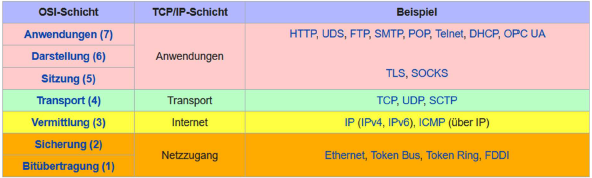
\includegraphics[width=\textwidth]{images/Netzwerkprotokolle_OSI-Schicht.PNG}
\caption[Netzwerkprotokolle: OSI-Schichten]{Netzwerkprotokolle: OSI-Schichten \protect \footnotemark}
\label{fig:OSISchichten}
\end{figure}
\footnotetext{Quelle: \url{https://de.wikipedia.org/wiki/Internetprotokollfamilie}, letzter Zugriff: 06. April 2021}

\newpage

\begin{table}[tbt]
\caption[Kurzbeschreibung der OSI-Schichten]{Kurzbeschreibung der OSI-Schichten \cite{ekOSI}}
\label{tab:OSISchichtenbeschreibung}
\begin{center}
    \begin{tabular}{ l  p{8cm} }
    \toprule
     OSI-Schicht & Aufgabe \\ 
     \midrule
        
    Anwendungen & Funktionen für Anwendungen, sowie die Dateneingabe und -ausgabe. \\

    Darstellung & Umwandlung der systemabhängigen Daten in ein unabhängiges Format.  \\

    Sitzung & Steuerung der Verbindungen und des Datenaustauschs.  \\

    Transport & Zuordnung der Datenpakete zu einer Anwendung. \\
    
	Vermittlung & Routing der Datenpakete zum nächsten Knoten. \\
	
	Sicherung & Fehlererkennungsmechanismen / Segmentierung der Pakete in Frames und Hinzufügen von Prüfsummen.  \\
    
    Bitübertragung & Umwandlung der Bits in ein zum Medium passendes Signal und physikalische Übertragung.\\ 
    \bottomrule
    \end{tabular}
\end{center}
\end{table}

\noindent
\hangindent1cm
\textbf{IP:}
In der Vermittlungsschicht des OSI-Schichtenmodells findet, unabhängig vom Über\-tra\-gungs\-mediums und der genutzten Topologie, die logische Adressierung der Endgeräte statt. Das geläufigste Protokoll dafür ist das Internet Procotol (IP). Jedem am Netz verbundenen Teilnehmer wird eine IP-Adresse zugewiesen. Die bekannteste Notation ist die 32\,Bit lange IPv4-Adressen und die IPv6-Adressen mit einer Größe von 128\,Bit.\\

\noindent
\hangindent1cm
\textbf{TCP/UDP:}
In der Transportschicht wird eine Ende-zu-Ende-Kommunikation ermöglicht. 
Sie ist das Bindeglied zwischen den anwendungsorientierten und den transportorientierten Schichten. 
Die geläufigsten Protokolle sind das User Datagram Protocol (UDP) und das Transmission Control Protocol (TCP).
UDP ist verbindungslos und daher unzuverlässiger, ist aber durch weniger Overhead belastet.
TCP hingegen ist verbindungsorientiert und dadurch zuverlässiger beim Datentransfer.
Jedes netzwerkfähige Gerät enthält eine Vielzahl von Ports, die primär zur
Unterscheidung zwischen Datenströmen aus Anwendungen bei Netzwerkverbindungen
genutzt werden. Anhand des genutzten Ports bei Netzwerkanfragen
wissen Webserver, welches Protokollverfahren genutzt werden soll.

\noindent
\subsubsection{HTTP}
Das Hypertext Transfer Protocol, kurz HTTP, ist ein zustandloses Protokoll zur Übertragung von Daten auf der Anwendungsschicht. \\

\noindent
\hangindent1cm
\textbf{Kommunikation:}
Unter einer Nachricht versteht man in HTTP die Kommunikationseinheiten zwischen dem Zentralrechner (Server) und dem, der einen Dienst vom Server abruft (Client). 
Man unterscheidet dabei zwischen der Anfrage (Request) vom Client an den Server und der Antwort (Response) als Reaktion vom Server zum Client. 
\newline
\noindent
Eine Nachricht besteht aus dem Nachrichtenkopf (Message Header, kurz Header) und dem Nachrichtenrumpf (Message Body, kurz Body). 
Der Header enthält generelle Informationen über die Nachricht wie zum Beispiel den Methodentyp, das Datenformat, den genutzten Kompressionsalgorithmus, die Länge der Nachricht oder die verwendete Codierung im Body. 
\newline
\noindent
In Abbildung \ref{fig:HTTPNachricht} ist der Aufbau der HTTP-Nachrichten dargestellt.
Die erste Zeile des Nachrichtenkopfs ist dreiteilig und besteht bei der Anfrage aus dem Namen der Anfragemethode, dem Pfad zur angeforderten Ressource (Uniform Resource Locator, kurz URL) und der verwendet HTTP-Version. Die Anfangszeile einer HTTP-Antwort dagegen besteht zunächst aus der verwendeten HTTP-Version, gefolgt von dem zweiteiligem Status-Code. 
Der Anfangszeile beider Nachrichtentypen folgt eine Reihe von Headerzeilen, wobei jede Zeile aus einem Schlüsselwort/Wert-Paar besteht und die für die Datenübertragung wichtigen Informationen übergibt. 
Der Nachrichtenrumpf, der mit den Nachrichtenkopf über einen Zeilenumbruch syntaktisch voneinander getrennt wird, enthält schließlich die Nutzdaten.
\newline

\begin{figure}[tbt]
\centering
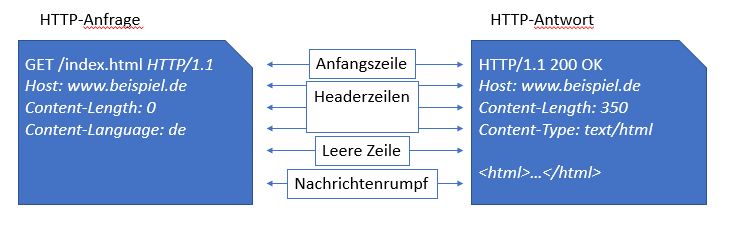
\includegraphics[width=\textwidth]{images/netzwerkprotokolle_http.PNG}
\caption{HTTP-Nachrichtenaufbau}
\label{fig:HTTPNachricht}
\end{figure}

\noindent
\hangindent1cm
\textbf{Methoden:}
HTTP bietet fest definierte Standard-Methoden für Anfragen, die für verschiedene Aufgaben gedacht sind. Im Folgenden werden die wichtigsten Methoden beschrieben:
\begin{itemize}
{\setlength\itemindent{1cm}\item\textit{GET} ist die gebräuchlichste Methode. Sie fordert vom Server eine Ressource, die bei Erfolg in der Antwort im Body zurückgegeben wird.}
		
		\item \textit{POST} ist für die Änderung oder Erzeugung einer Ressource vorgesehen. Dafür werden bei der Anfrage zus"atzlich Daten im Body der Nachricht übertragen.
		
		\item \textit{PUT} dient dazu, eine Ressource zu verändern, oder bei Nichtexistenz zu erstellen.
	
		\item \textit{PATCH} ändert eine bestehende Ressource ohne diese wie bei PUT vollständig zu ersetzen. 
		
		\item \textit{DELETE} löscht die angegebene Ressource auf dem Server.
		
		\item \textit{OPTIONS} liefert eine Liste von Methoden und Merkmale, die vom Server unterstützt werden.
		
\end{itemize}
\newpage
\noindent
\hangindent1cm
\textbf{Status-Codes:}
HTTP-Antworten senden in der Anfangszeile ihrer Nachricht Status-Codes. Die Angabe ist zweiteilig und besteht aus einer standardisierten Statuskennzahl sowie einer kurzen textuellen Beschreibung, die zusammen Auskunft über den Bearbeitungszustand der zugehörigen Anfrage geben. Tabelle \ref{tab:HTTPStatuscode} stellt die Status-Codes und ihre Beschreibungen anhand von Beispielen dar. \newline

\begin{table}[tbt]
\caption{HTTP Statuscodebeschreibungen}
\label{tab:HTTPStatuscode}
\begin{center}
    \begin{tabular}{ l  l   p{8cm} }
    \toprule
    Typ & Status-Code & Beispiele \\
    \midrule
    
    Informational & 1xx & 100 Continue, 101 Switching\\

    Success & 2xx & 200 OK, 201 Created, 202 Accepted  \\

	Redirection & 3xx & 300 Multiple Choice, 301 Moved Permanently  \\

    Client Error & 4xx & 400 Bad Request, 403 Forbidden\\ 

    Server Error & 5xx & 500 Internal Server Error \\
    \bottomrule
    \end{tabular}
\end{center}
\end{table}

\subsubsection{HTTPS}
Das HTTP-Protokoll hat den großen Nachteil, dass die Nachrichten unverschlüsselt und ungesichert übertragen werden. 
Die Daten können bei der Übertragung von Dritten empfangen, gelesen und verändert werden. Hypertext Transfer Protocol Secure, kurz HTTPS, soll dem entgegenwirken und die Sicherheit bei der Kommunikation gewährleisten. 
Dafür dienen zwei Konzepte:
\newline

\noindent
\noindent
Ersteres ist das Verschlüsseln der Kommunikation von Sender und Empfänger. Die zugrundeliegende Technik nennt sich Transport Layer Security (TLS), ist aber auch als Secure Sockets Layer (SSL) bekannt. Die Idee dahinter ist, dass jeder Teilnehmer der Kommunikation einen öffentlich bekannten Schlüssel (Public Key) und einen geheimen, nicht-öffentlichen Schlüssel (Private Key) besitzt. Über den Public-Key des Empfängers verschlüsselt der Sender seine Nachricht. Diese kann nur über den Private-Key des Empfängers entschlüsselt werden, der vom Empfänger nicht weitergegeben werden sollte.
\newline

\noindent
Das zweite Konzept von HTTPS ist die Webserver-Authentifizierung. Ein Zertifikat, das zu Beginn der Kommunikation an den Webclient gesendet wird, bescheinigt die Vertrauens"-würdig"-keit des Servers. Dafür vertrauen Browser- und Betriebssystemhersteller bestimmten Zertifizierungsstellen, deren Zertifikate sie in ihrem Browser bzw. Betriebssystem hinterlegen. Die Kommunikation zwischen Webserver und Webclient findet folglich erst nach vollständiger Authentifizierung statt.
